\chapter{Łańcuchy Markowa}

\section{Podstawowe pojęcia i definicje}
W tym podrozdziale dokonamy przeglądu kliku podstawowych definicji z teorii prawdopodobieństwa, które będą potrzebne przy rozważaniach opisanych w kolejnych częściach rozdziału pierwszego.

\subsection{Przestrzeń i funkcja mierzalna}

\begin{definicja}
	$\sigma$-algebrą podzbiorów zbioru $\Omega$ nazywamy rodzinę $\mathcal{F} \subset	2^{\Omega}$ spełniającą następujące warunki.
	\begin{itemize}
		\item $\emptyset, \Omega \in \mathcal{F}$.
		\item Jeżeli $ \mathcal{A} \in \mathcal{F}$, to również $\mathcal{A^{C}} \in \mathcal{F}$.
		\item Jeżeli $ \mathcal{A}_{1} , \mathcal{A}_{2} , ..., \in F$, to $\bigcap_{j=1}^{\infty} A_{j} \in \mathcal{F}$	
	\end{itemize}
\end{definicja}

\begin{przyklad}
	Przykłady $\sigma$-algebr:
	\begin{itemize}
		\item Rodzina wszystkich podzbiorów zbioru $\Omega$ tworzy $\sigma$-algebrę: $\mathcal{F} = 2^{\Omega}$,
		\item Rodzina $\mathcal{F}$ złożona z $\{\emptyset, \Omega \}$ tworzy $\sigma$-algebrę,
		\item Niech $\mathcal{R} = \{ A_{1}, A_{2}, ..., A_{n} \}$ skończone rozbicie przestrzeni $\Omega$, tj. $\Omega = \bigcup\limits_{j=1}^{n} A_{i}$ i zbiory $A_{j}$ są parami rozłączne: $A_{i} \cap A_{j} = \emptyset$, jeśli $i \neq j$. Wtedy $\mathcal{F}$ złożona z sum rozłącznych elementów rozbicia $\mathcal{R}$ jest $\sigma$-algebrą.		
	\end{itemize}
\end{przyklad}


\begin{definicja}
	Przestrzenią mierzalną nazywamy parę $(\Omega, \mathcal{F})$, gdzie $\Omega$ jest niepustym zbiorem, a $\mathcal{F}$ jest $\sigma$-algebrą podzbiorów zbioru $\Omega$.
\end{definicja}

\begin{przyklad}
	Niech $ \Omega $ będzie niepustym zbiorem. Następujące pary $(\Omega, \mathcal{F})$ stanowią przykłady przestrzeni mierzalnych:
	\begin{itemize}
	
		\item $(\Omega, 2^{\Omega})$ - tworzy $\sigma$-algebrę
		\item $(\Omega, \{ \emptyset, \Omega\})$ - tworzy $\sigma$-algebrę
		\item $(\Omega, \{ \emptyset, \Omega, A, \Omega \backslash A \})$ dla dowolnego $ A \subseteq \Omega$ - tworzy $\sigma$-algebrę

	\end{itemize}
	
\end{przyklad}

\begin{przyklad}
	Rodzina wszystkich podzbiorów zbioru $\Omega$ jest $\sigma$-algebrą w $\Omega$
\end{przyklad}

Symbolem $\mathbb{R}^{1}$ oznaczmy zbiór liczb rzeczywistych dodatnich.
\begin{definicja}
	Funkcję $f:  (\Omega, \mathcal{F}) \to \mathbb{R}^{1}$ nazywamy mierzalną, jeśli dla każdego $a \in \mathbb{R}^{1}$
\end{definicja}
{\centering
	$\{f \le a\} = \{ \omega; f(\omega) \le a \} \in \mathcal{F}. $\par
}

\begin{definicja}
	Podzbiory borelowskie $\mathbb{R}^{1}$ to elementy $\sigma$-algebry generowanej przez podzbiory otwarte (równoważnie: domknięte) zbioru $\mathbb{R}^{1}$.  $\sigma$-algebrę zbiorów borelowskich oznaczamy symbolem $\mathcal{B}^{1}$.																
\end{definicja}

\begin{przyklad}
Z definicji wiemy, że każdy zbiór otwarty jest zbiorem borelowskim, a także zbiór domknięty, jako uzupełnienie zbioru otwartego. Zbiorami borelowskimi są również zbiory 1-punktowe. Zbiór liczb wymiernych $Q \subset R$ jest borelowski jako przeliczalna suma zbiorów 1-punktowych, zatem liczby niewymierne $ R \setminus Q$ także stanowią zbiór borelowski.
\end{przyklad}

\subsection{Zmienna losowa}

\begin{definicja}
	Przestrzenią probabilistyczną nazywamy trójkę  $(\Omega, \mathcal{F}, \mathcal{P})$, gdzie
	\begin{itemize}
		\item $\Omega$ jest zbiorem "zdarzeń elementarnych" (elementy $\omega$ zbioru $\Omega$ nazywamy $\textit{zdarzeniami elementarnymi}$).
		\item $\mathcal{F}$ jest $\sigma$-algebrą podzbiorów zbioru $\Omega$. Elementy $\mathcal{F}$ nazywane są $\textit{zdarzeniami}$.
		\item $P: \mathcal{F} \rightarrow \lbrack 0, 1 \rbrack$ jest prawdopodobieństwem na $(\Omega, \mathcal{F})$.
	\end{itemize}
\end{definicja}

\begin{przyklad}
	Aby obliczyć szansę dowolnego zdarzenia $A$ trzeba określić liczbę zdarzeń sprzyjających oraz liczbę wszystkich możliwych zdarzeń. Do obliczenia prawdopodobieństwa korzysta się z wzoru:
	\begin{center}
		$ P (A) = \frac{\#A}{\#\Omega} = \frac{ ilosc \ elemetów \ w \ zbiorze \ A }{ilosc \ elemetów \ w \ zbiorze \ \Omega} $
	\end{center}
	gdzie:
	\begin{itemize}
		\item $\#A$ to liczba zdarzeń sprzyjających
		\item $\#\Omega$ to liczba wszystkich możliwych zdarzeń
	\end{itemize}
	Rozważmy przykład, w którym można zastosować powyższe rozważania. 
	Należy obliczyć prawdopodobieństwo, że w rzucie kostką wypadnie liczba oczek mniejsza od 5. \\
	Dane:
	\begin{itemize}
		\item zdarzeniem losowym jest rzut kostką
		\item $\Omega$ - zbiór wszystkich możliwych zdarzeń. $\Omega = \{1, 2, 3, 4, 5, 6\}$.
		\item $A$ - zbiór wyników, których liczba oczek jest mniejsza od 5. $A = \{1, 2, 3, 4\}$.
		\item $\#\Omega = 6$ - zbiór $\Omega$ liczy 6 elementów
		\item $\#A = 4$ - zbiór $A$ liczy 4 elementy
	\end{itemize}
	Zatem prawdopodobieństwo zdarzenia $A$ jest liczone według wzoru:
	\begin{center}
		$P(A) = \frac{A}{\Omega} = \frac{4}{6} = \frac{2}{3}$
	\end{center}
	
\end{przyklad}

\begin{definicja}
	Zmienną losową na przestrzeni $(\Omega, \mathcal{F}, \mathcal{P})$ nazywamy funkcję $X:  (\Omega, \mathcal{F}) \to \mathbb{R}^{1}$ o własności 
	\begin{center}
		$\mathnormal{ X^{-1} \left(  -\infty, u \rbrack
			\right) \in \mathcal{F}, u \in \mathbb{R}^{1}}$.
	\end{center}
\end{definicja}

\begin{przyklad}
	Niech $\Omega$ będzie zbiorem wszystkich możliwych wyników przy pojedynczym rzucie dwiema kostkami do gry. Zbiór $\Omega$ składa się z 36 możliwych wyników i oznaczmy go: $\Omega = \{ (i,j); 1 \le i,j \le 6 \} $. Rozważmy funkcję $X: \Omega \rightarrow \mathbb{R}^{1}$. Określoną wzorem:
 
		$$\forall_{(i,j) \in \Omega }\; \space \space X(i,j)=i+j $$
 	
	 Symbolem $\mathcal{F}$ oznaczmy wszystkie podzbiory zbioru $\Omega$. Wówczas trójka $(\Omega, \mathcal{F}, \mathcal{P})$ gdzie $P: \mathcal{F} \rightarrow \lbrack 0, 1 \rbrack$ określona wzorem:
	 \begin{center}
	 		$ P (A) = \frac{\#A}{36} $
	 \end{center}
	 jest przestrzenią probabilistyczną, a funkcja $X$ jest zmienną losową.
	  
\end{przyklad}

\begin{przyklad}
	Rozważmy przestrzeń $(\Omega, \mathcal{F}, \mathcal{P})$ w której:
	\begin{itemize}
		\item $\Omega$  - jest niepustym zbiorem,
		\item $P: \mathcal{F} \rightarrow \lbrack 0, 1 \rbrack$ jest prawdopodobieństwem na $(\Omega, \mathcal{F})$
		\item $P(\emptyset) = 0$
		\item $P(\Omega) = 1$
		\item $P(A) = p$ dla $0 \le p \le 1$ \\ \newline
		Wówczas:
		\item $P(\Omega \setminus A) = 1-p$
	\end{itemize}
\end{przyklad}



\section{Cechy Łańcuchów Markowa}

Procesem Markowa to ciąg zmiennych losowych (ciąg zdarzeń), w którym prawdopodobieństwo każdego zdarzenia zależy jedynie od wyniku poprzedniego. Procesem stochastycznym nazywamy proces, w którym teoria prawdopodobieństwa używana jest do modelowania losowych zjawisk. Łańcuch Markowa to proces Markowa, który zdefiniowany jest na dyskretnej przestrzeni stanów, jest to jeden z procesów stochastycznych.

\begin{definicja}
	
	Łańcuchem Markowa o zbiorze stanów ${S}$ $\mathbb{R}$\ nazywamy ciąg zmiennych losowych $X_{0}$, $X_{1}$, $X_{2}$,... taki, że: \\
	 $$\mathnormal{P \left( X_{n} = x_{n}|X_{n-1} = x_{n-1} \wedge X_{n-2} = x_{n-2}
		\wedge ... \wedge X_{0} = x_{0} \right) = P \left( X_{n} = x_{n}|X_{n-1} = x_{n-1}\right)  = p_{x_{n-1}}, x_{n}}$$ 
	dla każdego $\mathnormal{n > }$ 0 i ciągu stanów $\mathnormal{x_{0}, x_{1}, ..., x_{n}} \in {S}$.
	
\end{definicja} 

Dziedzina zmiennych losowych nazywana jest przestrzenią stanów. Pojedynczy stan opisywany jest przez ${X_{t}}$ w chwili $t$. Stany w Łańcuchu Markowa wzajemnie od siebie zależą, możemy powiedzieć, że zmienna ${X_{t}}$ zależy tylko od zmiennej ${X_{t-1}}$. Nie oznacza to, że ${X_{t}}$ jest niezależna od $\mathnormal{X_{0}, X_{1}, ..., x_{t-2}}$  
 
\begin{definicja}
	Macierzą przejścia w jednym kroku łańcucha Markowa nazywamy macierz $\mathnormal{M = (p_{i,j})_{i,j \in S}}$. Wiersze macierzy przejścia łańcucha Markowa sumują się do 1, czyli $\sum_{j} p_{i,j} = 1 $.
\end{definicja}

Liczby $p_{i,j}$, które występują  w definicji Łańcucha Markowa to prawdopodobieństwa przejścia w jednym kroku. Jeżeli w danej chwili Łańcuch Markowa jest w stanie $i$, to z prawdopodobieństwem $p_{i,j}$ znajdzie się w następnej chwili w stanie $j$ .

\[
M=
\begin{bmatrix}
	p_{0,0}(t) & p_{0,1}(t) & p_{0,2}(t) & \dots  & p_{0,j}(t) \\
	p_{1,0}(t) & p_{1,1}(t) & p_{1,2}(t) & \dots  & p_{1,j}(t) \\
	\vdots & \vdots & \vdots & \ddots & \vdots \\
	p_{i,j}(t) & x_{i,j}(t) & p_{i,j}(t) & \dots  & p_{i,j}(t)
\end{bmatrix}
\]

$$ \text{Macierz przejścia}$$


\begin{przyklad}
	Dany jest zbiór stanów $S = \{A, B\}$, w tej przestrzeni stanów można zdefiniować 4 możliwe przejścia. Macierz przejścia $M$ wygląda następująco:
	\[
	M =
	\begin{bmatrix}
	0.3 & 0.7 \\
	0.4 & 0.6	
	\end{bmatrix}
	\]
Liczba 0.4 z pierwszej kolumny drugiego wiersza mówi, że istnieje czterdziesto procentowe prawdopodobieństwo, że ze stanu $A$ dojdziemy do stanu $B$. Następnie, ze stanu $B$ istnieje sześćdziesięcio procentowe prawdopodobieństwo, że zostanie osiągnięty z powrotem stan $B$.
Macierzy $M$ odpowiada automat z przejściami przedstawiony poniżej. 	

\begin{center}
	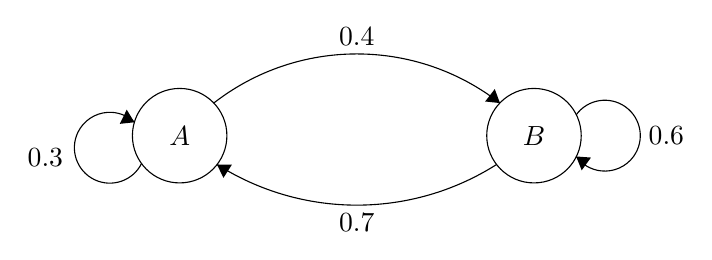
\begin{tikzpicture}[scale=0.2]
	\tikzstyle{every node}+=[inner sep=0pt]
	\draw [black] (19.6,-21) circle (3);
	\draw (19.6,-21) node {$A$};
	\draw [black] (42.1,-21) circle (3);
	\draw (42.1,-21) node {$B$};
	\draw [black] (21.764,-18.93) arc (127.91446:52.08554:14.786);
	\fill [black] (39.94,-18.93) -- (39.61,-18.04) -- (39,-18.83);
	\draw (30.85,-15.31) node [above] {$0.4$};
	\draw [black] (39.727,-22.829) arc (-57.55971:-122.44029:16.549);
	\fill [black] (21.97,-22.83) -- (22.38,-23.68) -- (22.92,-22.84);
	\draw (30.85,-25.91) node [below] {$0.7$};
	\draw [black] (44.78,-19.677) arc (144:-144:2.25);
	\draw (49.35,-21) node [right] {$0.6$};
	\fill [black] (44.78,-22.32) -- (45.13,-23.2) -- (45.72,-22.39);
	\draw [black] (17.184,-22.759) arc (-26.20682:-314.20682:2.25);
	\draw (12.23,-22.39) node [left] {$0.3$};
	\fill [black] (16.73,-20.15) -- (16.24,-19.35) -- (15.8,-20.25);

	\end{tikzpicture}
\end{center}
	
	
\end{przyklad}

Inną równoważną definicją jest trójka $ \langle Q,\pi, p \rangle$, którą definiuje się w sposób następujący:

\begin{definicja}
	Łańcuchem Markowa nazywamy trójkę $ \langle Q,\pi, p \rangle$, gdzie:
	\begin{itemize}
		\item $Q$ jest przestrzenią stanów,
		\item $p: Q \times Q \rightarrow \lbrack 0, 1 \rbrack$ - prawdopodobieństwo osiągnięcia stanu w momencie przejścia,
		\item $\pi: Q \rightarrow \lbrack 0, 1 \rbrack$ - prawdopodobieństwo osiągnięcia stanu inicjalizującego. 
	\end{itemize}
	
	Ponadto muszą zachodzić warunki:
	\begin{itemize}
		\item dla $q_{i} \in Q$, $\sum_{q_{j} \in Q} a(q_{i}, q_{j}) = 1$,
		\item $\sum_{q \in Q} \pi(q) = 1.$
	\end{itemize}	
\end{definicja}

\begin{przyklad}
	Student raz w tygodni bierze udział w zajęciach z rachunku prawdopodobieństwa. Na każde zajęcia przychodzi przygotowany bądź nie. Jeśli w danym tygodniu jest przygotowany, to w następnym jest przygotowany z prawdopodobieństwem 0.7. Jeśli natomiast w danym tygodniu nie jest przygotowany, to w następnym jest przygotowany z prawdopodobieństwem 0.2. Interesujące są pytania na odpowiedzi:
	
	\begin{enumerate}
		\item Jeśli student jest w tym tygodniu nieprzygotowany, to ile tygodni musimy średnio czekać aż będzie przygotowany?
		\item Na dłuższą metę, jak często student jest przygotowany?
	\end{enumerate}
	
	Wyróżniamy tutaj dwa stany: 1 - student jest przygotowany, oraz 2 - student nie jest przygotowany. Na podstawie danych można skonstruować macierz przejścia:\newline
	\[
	M = 
	\begin{bmatrix}
		0.7 & 0.3 \\
		0.2 & 0.8 
	\end{bmatrix}\\
	\]
	Dane: zbiór stanów $S \subseteq \mathcal{R}$, $S = \{0,1\} $. Prawdopodobieństwa zdarzeń przedstawiają się w sposób następujący: \\ \\ 
	$P(X_{t_{2}} = 0 | X_{t_{2}} = 1) = 0.3 = p_{1,0}$ \\
	$P(X_{t_{2}} = 1 | X_{t_{2}} = 1) = 0.7 = p_{1,1}$ \\
	$P(X_{t_{2}} = 1 | X_{t_{2}} = 0) = 0.2 = p_{0,1}$ \\
	$P(X_{t_{2}} = 0 | X_{t_{2}} = 0) = 0.8 = p_{0,0}$ \\
		
	Wiersze macierzy $M$ zgodnie z definicją macierzy przejścia sumują się do 1. 
	Przypuśćmy, że znany jest rozkład zmiennej $\mathnormal{X_{t}}$ czyli prawdopodobieństwo tego, że w chwili $\mathnormal{t}$ znajdujemy się w poszczególnych stanach. Trzeba znaleźć rozkład zmiennej $\mathnormal{X_{t+1}}$ oraz ogólniej rozkład zmiennej $\mathnormal{X_{t+s}}$. Taki rozkład można łatwo znaleźć korzystając z macierzy $\mathnormal{M}$. \\
	Ze wzoru na prawdopodobieństwo całkowite wynika:
	\begin{center}
		$P(X_{t+1} = a) = \sum_{b \in \mathcal{S}} P(X_{t} = b)P(X_{t+1} = a | X_{t} = b) = \sum_{b \in \mathcal{S}} \pi(t)_{b} M_{b,a}$
	\end{center}
	Mówiąc prościej, mamy tutaj do czynienia z mnożeniem macierzy przez wektor, co można zapisać: $\pi(t) \cdot M = \pi(t+1)$
	
\end{przyklad}

\begin{przyklad}
Firmy ubezpieczeniowe wykorzystują łańcuchy Markowa do obliczenia ile rzeczywiście pieniędzy pobierają od swoich klientów. Przykładowym modelem, na którym można to zbadać jest model podsumowujący stan zdrowia człowieka w cyklu miesięcznym.\\

Dane: zbiór stanów $S \subseteq \mathcal{R}$, $S = \{1, 2, 3\} $. gdzie $1$ - oznacza osobę zdrową, $2$ - oznacza osobę chorą, $3$ - oznacza śmierć. Prawdopodobieństwa zdarzeń przedstawiają się w następujący sposób. \\ \\ 
$P(X_{n} = 1 | X_{n} = 2) = 0.3 = p_{2,1}$ \\
$P(X_{n} = 1 | X_{n} = 1) = 0.6 = p_{1,1}$ \\
$P(X_{n} = 2 | X_{n} = 1) = 0.8 = p_{1,2}$ \\
$P(X_{n} = 2 | X_{n} = 2) = 0.1 = p_{2,2}$ \\

Prawdopodobieństwa można zobrazować w postaci automatu z przejściami:

\begin{center}
	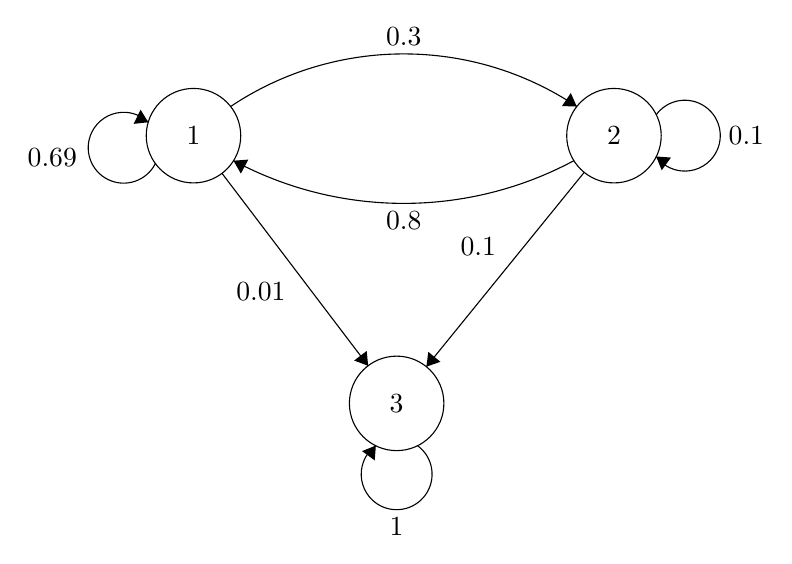
\begin{tikzpicture}[scale=0.2]
	\tikzstyle{every node}+=[inner sep=0pt]
	\draw [black] (19.9,-21.2) circle (3);
	\draw (19.9,-21.2) node {$1$};
	\draw [black] (46.6,-21.2) circle (3);
	\draw (46.6,-21.2) node {$2$};
	\draw [black] (32.8,-38.2) circle (3);
	\draw (32.8,-38.2) node {$3$};
	\draw [black] (22.257,-19.348) arc (123.80513:56.19487:19.759);
	\fill [black] (44.24,-19.35) -- (43.86,-18.49) -- (43.3,-19.32);
	\draw (33.25,-15.51) node [above] {$0.3$};
	\draw [black] (44.057,-22.787) arc (-61.79923:-118.20077:22.868);
	\fill [black] (22.44,-22.79) -- (22.91,-23.61) -- (23.38,-22.72);
	\draw (33.25,-26) node [below] {$0.8$};
	\draw [black] (49.28,-19.877) arc (144:-144:2.25);
	\draw (53.85,-21.2) node [right] {$0.1$};
	\fill [black] (49.28,-22.52) -- (49.63,-23.4) -- (50.22,-22.59);
	\draw [black] (17.484,-22.959) arc (-26.20682:-314.20682:2.25);
	\draw (12.53,-22.59) node [left] {$0.69$};
	\fill [black] (17.03,-20.35) -- (16.54,-19.55) -- (16.1,-20.45);
	\draw [black] (21.71,-23.59) -- (30.99,-35.81);
	\fill [black] (30.99,-35.81) -- (30.9,-34.87) -- (30.1,-35.48);
	\draw (25.78,-31.1) node [left] {$0.01$};
	\draw [black] (44.71,-23.53) -- (34.69,-35.87);
	\fill [black] (34.69,-35.87) -- (35.58,-35.56) -- (34.81,-34.93);
	\draw (39.14,-28.27) node [left] {$0.1$};
	\draw [black] (34.123,-40.88) arc (54:-234:2.25);
	\draw (32.8,-45.45) node [below] {$1$};
	\fill [black] (31.48,-40.88) -- (30.6,-41.23) -- (31.41,-41.82);
	\end{tikzpicture}
\end{center}

Brakujące prawdopodobieństwa zostały wyliczone biorąc pod uwagę własność macierzy przejścia, w której wiersze sumują się do 1. \\
$p_{1,1} = 1 - p_{1,2} - p_{1,3}$ oraz $p_{2,2} = 1 - p_{2,1} - p_{2,3}$. Na podstawie powyższego łańcuchy Markowa można próbować odpowiedzieć na pytania:

\begin{itemize}
	\item Jaka jest długość życia obecnie zdrowej osoby?
	\item Jaka jest długość życia obecnie chorej osoby?
\end{itemize}

\end{przyklad}


\begin{przyklad}
 
	Niech dane będą dwie zmienne losowe $X_{0}, X_{1}$, gdzie $X_{0}$ oznaczać będzie pogodę słoneczną, a $X_{1}$ oznaczać będzie pogodę pochmurną. Dla ułatwienia wprowadźmy oznaczenia: $X_{0} - S$, $X_{1} - C$. Następnie przypiszmy prawdopodobieństwo wystąpienia pogody słonecznej równe $\frac{1}{2}$ oraz prawdopodobieństwo wystąpienia pogody pochmurnej równe $\frac{1}{2}$. Następnym krokiem będzie wygenerowanie losowej pogody na 356, gdzie taki rozkład można zaprezentować za pomocą symboli np. $S,S,C,C,S,S,S,C,S,C,S,C, ..., n$. Mając rozkład w postaci symboli można go zobrazować w postaci wykresu.
 
	
	\begin{figure}[H]
		\centering
		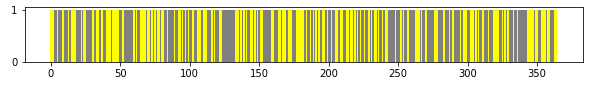
\includegraphics[width=0.7\linewidth]{wykres_pogoda}
		\caption[ ]{Wykres prawdopodobieństwa}
		\label{fig:wykrespogoda}
	\end{figure}
	Powyższa ilustracja obrazuje działanie modelu, pogoda każdego dnia jest niezależna od poprzednich dni, pobierana jest również z tego samego rozkładu. W następnym kroku wykorzystamy łańcuch Markowa i macierz przejścia aby uzależnić dany stan od poprzedniego. Łańcuch Markowa rozpocznie się w określonym stanie, a następnie pozostanie w tym samym stanie lub przejdzie do innego stanu na podstawie macierzy prawdopodobieństw:
	
	\[
	P = 
	\begin{bmatrix}
	0.7 & 0.3 \\
	0.2 & 0.8 
	\end{bmatrix}\\
	\]
	
	Z macierzy możemy odczytać, że prawdopodobieństwo zajścia dnia słonecznego pod warunkiem, że poprzedniego dnia był słoneczny dzień wynosi 0.7

\begin{figure}[H]
\begin{center}
	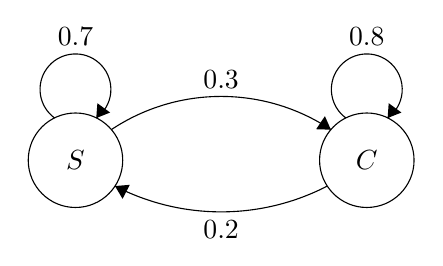
\begin{tikzpicture}[scale=0.2]
	\tikzstyle{every node}+=[inner sep=0pt]
	\draw [black] (23,-25.8) circle (3);
	\draw (23,-25.8) node {$S$};
	\draw [black] (41.5,-25.8) circle (3);
	\draw (41.5,-25.8) node {$C$};
	\draw [black] (21.677,-23.12) arc (234:-54:2.25);
	\draw (23,-18.55) node [above] {$0.7$};
	\fill [black] (24.32,-23.12) -- (25.2,-22.77) -- (24.39,-22.18);
	\draw [black] (40.177,-23.12) arc (234:-54:2.25);
	\draw (41.5,-18.55) node [above] {$0.8$};
	\fill [black] (42.82,-23.12) -- (43.7,-22.77) -- (42.89,-22.18);
	\draw [black] (25.276,-23.857) arc (123.65827:56.34173:12.583);
	\fill [black] (39.22,-23.86) -- (38.84,-23) -- (38.28,-23.83);
	\draw (32.25,-21.25) node [above] {$0.3$};
	\draw [black] (38.994,-27.439) arc (-62.66466:-117.33534:14.686);
	\fill [black] (25.51,-27.44) -- (25.99,-28.25) -- (26.45,-27.36);
	\draw (32.25,-29.58) node [below] {$0.2$};
	\end{tikzpicture}
	\caption{Graf prawdopodobieństw równoważny z macierzą przejść}
\end{center}
\end{figure}

Należy stworzyć zmienną losową dla każdego rzędu macierzy przejścia, zmienna losowa odpowiada prawdopodobieństwom przejść od stanu do stanu. 

\begin{figure}[H]
	\centering
	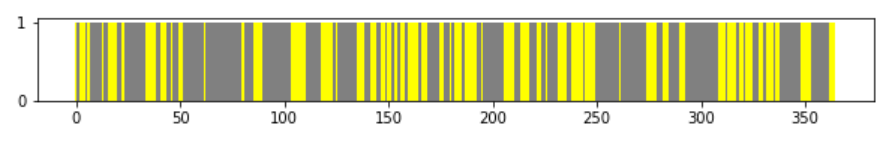
\includegraphics[width=0.7\linewidth]{pogoda_markov}
	\caption{Wykres prawdopodobieństwa po zastosowaniu łańcucha Markowa}
	\label{fig:pogodamarkov}
\end{figure}

Jak widać na ilustracji powyżej, po zastosowaniu łańcucha Markowa z zadaną macierzą przejścia wykres wygląda trochę inaczej. Za pomocą macierzy jesteśmy w stanie kontrolować długości danego stanu. Poniżej znajduje się pełen listing kodu programu, który realizuje powyższe rozważania.


\lstinputlisting[language=Python]{markov_chain_var_ex.py}


\end{przyklad}


\subsection{Pojęcia i własności łańcuchów}
	
	W teorii prawdopodobieństwa oraz statystyce rozważa się inne modele matematyczne, które bazują na probabilistyce i są trochę bardziej rozbudowane niż klasyczny łańcuch Markowa. Należy tutaj wymienić takie modele jak: łańcuchy Markowa wyższego rzędu, ukryte modele Markowa, łańcuchy Markowa mieszanego rzędu, łańcuchy Markowa wyższego rzędu, probabilistyczne skończone automaty. Poniżej zostaną przedstawione niektóre z nich.
	

	Rozpoczniemy od opisu ukrytych modeli Markowa. Ukryte modele Markowa (HMM, ang. hidden Markov models) są rozszerzeniem standardowej definicji łańcucha Markowa. Używane są głównie do modelowania związku między ukrytymi, a obserwowanymi sekwencjami. Ukrytym modelem Markowa jest łańcuch Markowa z dyskretnym rozkładem prawdopodobieństwa w każdym stanie. Dyskretne rozkłady prawdopodobieństwa definiują prawdopodobieństwa emisji określonego symbolu alfabetu w danym stanie. 

\begin{definicja}
	Ukrytym modelem Markowa nazywamy piątkę $ \langle \sum, Q, a, b, \pi  \rangle$ gdzie:
	\begin{itemize}
		\item $\sum$ jest skończonym alfabetem widocznych symboli,
		\item $Q$ jest skończonym zbiorem ukrytych stanów,
		\item $a: Q \times Q \rightarrow \lbrack 0, 1 \rbrack$ - prawdopodobieństwo osiągnięcia stanu pomiędzy stanami ukrytymi,
		\item $b: Q \times \sum \rightarrow \lbrack 0, 1 \rbrack$ - prawdopodobieństwo emisji określonego symbolu alfabetu w danym ukrytym stanie,
		\item $\pi: Q \rightarrow \lbrack 0, 1 \rbrack$ - początkowe prawdopodobieństwo ukrytych stanów.
	\end{itemize}
	Ponadto muszą zachodzić warunki:
	\begin{itemize}
		\item dla $q_{i} \in Q$, $\sum_{q_{j} \in Q} a(q_{i}, q_{j}) = 1$,
		\item $\sum_{q \in Q} \pi(q) = 1.$
	\end{itemize}	
	
	Oznaczmy sekwencję obserwacji i stanu ukrytego przez $X = X_{1}, ..., X_{n}$ i $s = s_{1}, ..., s_{n}$, gdzie $X_{i} \in \sum$ oraz $s_{i} \in Q$. W tym przypadku używamy następującej notacji:
	\begin{center}
		$\pi(q_{i}) = P(s_{1} = q_{i})$ \\
		$a(q_{i},q_{j}) = P(s_{t} = q_{j} | s_{t-1} = q_{i})$ \\
		$b(q_{j},X_{t}) = P(X_{t} | s_{t} = q_{j})$
	\end{center}  
	$P(x)$ jest prawdopodobieństwem zdarzenia, natomiast $P(x | y)$ jest prawdopodobieństwem zdarzenia $x$ pod warunkiem $y$.
\end{definicja}

\begin{przyklad}
	Klasycznym przykładem ukrytego łańcucha Markowa jest nieuczciwe kasyno do gry, które ma dwa rodzaje kości: uczciwą kostkę do gry (z prawdopodobieństwem $\frac{1}{6}$ wyrzuca się każda z sześciu możliwych wartości) oraz nieuczciwą kostkę (dla której prawdopodobieństwo wyrzucenia szóstki wynosi $\frac{1}{2}$, a dla pozostałych liczb $\frac{1}{10}$). Mamy do dyspozycji dwa stany: F (uczciwa kostka) i L (nieuczciwa kostka). Układ może zmieniać swój stan z pewnym prawdopodobieństwem, ale my stanu nie możemy zaobserwować (np. krupier zmienia kostki pod stołem). Jedynie widzimy ciąg liczb będących wynikiem rzutów kostką. To, którą kostką rzucamy zależy tylko i wyłącznie od stanu ukrytego łańcucha Markowa. Macierz przejścia zdefiniujemy następująco:
	\[
		P = 
		\begin{bmatrix}
		0.9 & 0.1 \\
		0.45 & 0.55 
		\end{bmatrix}\\
	\]
	gdzie $p_{F,F}=0.90$, $p_{L,L}=0.55$, $p_{F,L}=0.10$, $p_{L,F}=0.45$. Średni czas nieprzerwanego rzucania kostką uczciwą jest równy $\frac{1}{1-0.9} = 10$ okresów, a kostką fałszywą $ \frac{1}{0.55} = 2$. Chodź nie wiemy, którą kostką rzucamy to mamy o tym jednak jakąś informacje. Obserwujemy bowiem ciąg liczb będących wynikiem rzutów kostką. Macierz emisji dla tego przykładu wygląda następująco:
	
	\[
	\prod = 
	\begin{bmatrix}
	\frac{1}{6} & \frac{1}{6} & \frac{1}{6} & \frac{1}{6} & \frac{1}{6} & \frac{1}{6} \\
	\frac{1}{10} & \frac{1}{10} & \frac{1}{10} & \frac{1}{10} & \frac{1}{10} & \frac{1}{2} &
	\end{bmatrix}\\
	\]
		 
\end{przyklad}

\begin{przyklad}
	Ukryty łańcuch Markowa można również wykorzystać w muzyce do generowania akordów na podstawie progresji II V I. Progresja II V I jako następstwo akordów, jest wykorzystywana w szerokim zakresie gatunków muzycznych oraz jest podstawą harmonii jazzowej. W przykładzie będziemy rozważać progresje II V I dla akordów tonacji C-dur. Poszczególne akordy będą stanami w łańcuchu Markowa. Stany ukryte będą odpowiedzialne za typ akordu (minor7, major7, dominant7).
	
 \begin{figure}[H]
 	\centering
 	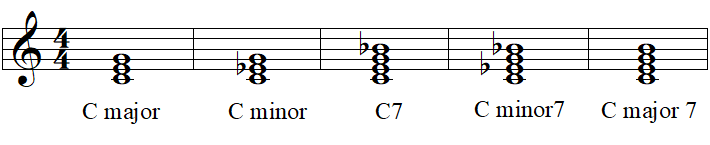
\includegraphics[width=0.7\linewidth]{akordy}
 	\caption{Podstawowe rodzaje akordów dla gamy C-dur}
 	\label{fig:akordy}
 \end{figure}

	W pierwszym kroku należy zdefiniować macierz przejścia dla stanów łańcucha Markowa. W przykładzie będą wykorzystane trzy stany, które będą odpowiadały nutą D, G, C - progresja II V I.
	
	\[
	P = 
	\begin{bmatrix}
	0.4 & 0.4 & 0.2 \\
	0.1 & 0.1 & 0.8 \\
	0.0 & 0.3 & 0.7 
	\end{bmatrix}\\
	\]
 
	Następnie musi zostać stworzona macierz emisji dla stanów ukrytych. Warstwa ukryta będzie odpowiedzialna za rodzaj akordu. Do dyspozycji będą trzy rodzaje akordów: minor7, major7, dominant7.
	
	\[
	M = 
	\begin{bmatrix}
	0.4 & 0.0 & 0.4 \\
	0.3 & 0.3 & 0.3 \\
	0.2 & 0.8 & 0.0 
	\end{bmatrix}\\
	\]
	 
	Dla danego stanu z macierzy $P$ będzie wybierany dany stan z macierzy $M$ z uwzględnieniem reguł łańcucha Markowa. Praktycznie zostanie to zrealizowane z użyciem języka Python. Pakiet o nazwie $hmmlearn$ zwolni nas z implementowania logiki Ukrytego Modelu Markowa, a za pomocą pakietu $music21$ będzie można wygenerować akordy na pięciolinii. 
	
	\begin{lstlisting}[caption={Ukryty Model Markowa z użyciem Pythona},captionpos=b]
 import numpy as np
 from hmmlearn import hmm
 from music21 import *
 
 environment.set("musescoreDirectPNGPath",     "/usr/bin/musescore")
 environment.set("musicxmlPath",     "/usr/bin/musescore")
 environment.set("midiPath",     "/usr/bin/lilypond")
 
 conv = converter.subConverters.ConverterLilypond()
 
 
 transmat = np.array([[0.4, 0.4, 0.2],
 [0.1, 0.1, 0.8],
 [0.0, 0.3, 0.7]])
 
 start_prob = np.array([1.0, 0.0, 0.0])
 
 emission_probs = np.array([[0.4, 0.0, 0.4],
 [0.3, 0.3, 0.3],
 [0.2, 0.8, 0.0]])
 
 chord_model = hmm.MultinomialHMM(n_components=2)
 
 chord_model.startprob_ = start_prob
 
 chord_model.transmat_ = transmat
 chord_model.emissionprob_ = emission_probs
 X, Z = chord_model.sample(10)
 
 state2name = {}
 state2name[0] = 'D'
 state2name[1] = 'G'
 state2name[2] = 'C'
 chords = [state2name[state] for state in Z]
 
 obj2name = {}
 obj2name[0] = 'min7'
 obj2name[1] = 'maj7'
 obj2name[2] = '7'
 
 observations = [obj2name[item] for sublist in X for item in sublist]
 chords = [''.join(chord) for chord in zip(chords, observations)]
 
 
 # create some chords for II, V, I
 d7 = chord.Chord(['D4', 'F4', 'A4', 'C5'])
 dmin7 = chord.Chord(['D4', 'F-4', 'A4', 'C5'])
 dmaj7 = chord.Chord(['D4', 'F#4', 'A4', 'C#5'])
 
 c7 = d7.transpose(-2)
 cmin7 = dmin7.transpose(-2)
 cmaj7 = dmaj7.transpose(-2)
 
 g7 = d7.transpose(5)
 gmin7 = dmin7.transpose(5)
 gmaj7 = dmaj7.transpose(5)
 print(g7.pitches)
 
 stream1 = stream.Stream()
 stream1.repeatAppend(dmin7, 1)
 stream1.repeatAppend(g7, 1)
 stream1.repeatAppend(cmaj7, 1)
 stream1.repeatAppend(cmaj7, 1)
 print(stream1)
 
 name2chord = {}
 name2chord['C7'] = c7
 name2chord['Cmin7'] = cmin7
 name2chord['Cmaj7'] = cmaj7
 
 name2chord['D7'] = d7
 name2chord['Dmin7'] = dmin7
 name2chord['Dmaj7'] = dmaj7
 
 name2chord['G7'] = g7
 name2chord['Gmin7'] = gmin7
 name2chord['Gmaj7'] = gmaj7
 hmm_chords = stream.Stream()
 
 for c in chords:
 	hmm_chords.repeatAppend(name2chord[c], 1)
 
 hmm_chords.show()
	\end{lstlisting}
	W przykładzie użyto 10 iteracji. Wynikiem działania programu jest sekwencja akordów przedstawiona poniżej:
	
	\begin{figure}[H]
		\centering
		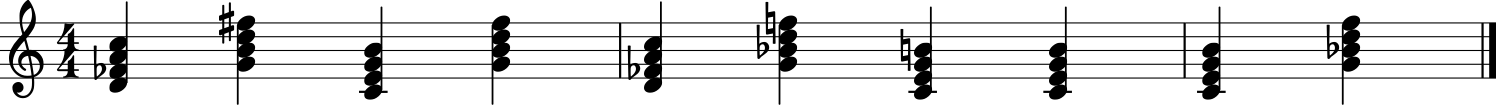
\includegraphics[width=0.7\linewidth]{hmm_music_notes}
		\caption{Wygenerowane akordy z użyciem ukrytego modelu Markowa}
		\label{fig:hmmmusicnotes}
	\end{figure}
	
	
	
\end{przyklad}

Powyższy kod został wzbogacony o interfejs użytkownika, w którym można definiować wartości macierzy prawdopodobieństw i emisji.

\begin{figure}[H]
	\centering
	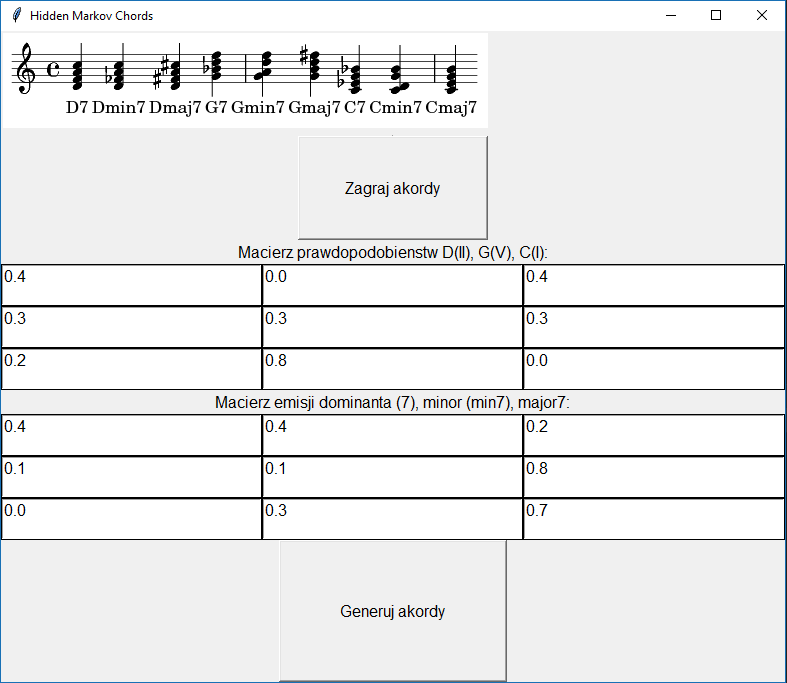
\includegraphics[width=0.7\linewidth]{hidden_markov_python}
	\caption{Interfejs aplikacji, która wykorzystuje ukryte modele Markowa do generowania akordów}
	\label{fig:hiddenmarkovpython}
\end{figure}


\begin{figure}[H]
	\centering
	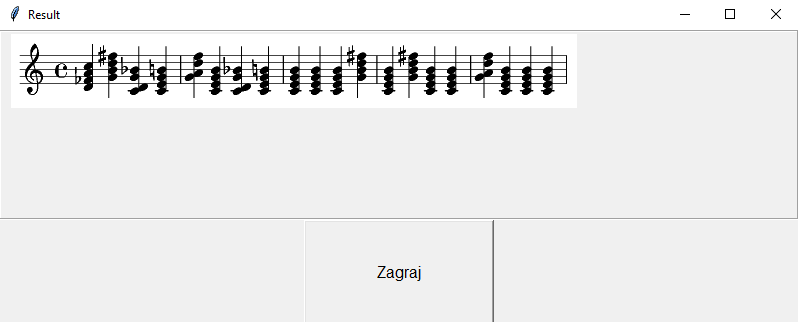
\includegraphics[width=0.7\linewidth]{hidden_markov_python_result}
	\caption{Wygenerowane akordy na podstawie zadanych macierzy}
	\label{fig:hiddenmarkovpythonresult}
\end{figure}

W programie wykorzystano bibliotekę music21, która posłużyła do zapisu nutowego oraz zapisu nut do pliku. Algorytm ukrytego modelu Markowa pochodzi z biblioteki hmmlearn.

Możemy powiedzieć, że standardowe Łańcuchy Markowa maja pamięć długości 1 ponieważ n-ty stan zależy tylko i wyłącznie od stanu poprzedniego. Przeciwieństwo stanowią Łańcuchy Markowa wyższego rzędu (ang. Higher Order Markov Chains), które mają pamięć większą niż jeden. 

\begin{definicja}
	Łańcuch Markowa N-tego rzędu definiujemy w następujący sposób:
	\begin{center}
		
		$P(q_{t} | q_{t-1}, q_{t-2}, ..., q_{1}) = P(q_{t} | q_{t-1}, ..., q_{t-min(t-1, N)})$
		
	\end{center}
	Jeżeli $t \leq N$ to $q_{t}$ jest stanem startowym oraz nadmierne stany $q_{t}$ gdzie $t \le 0$ są reprezentowane przez puste słowo $\lambda$. W przypadku Łańcucha Markowa N-tego rzędu będziemy używać zapisu $a(q_{t-N}, ..., q_{t-1}, q_{t})$ zamiast $a(q_{t-1}, q_{t})$ aby wskazać prawdopodobieństwa przejścia. 
\end{definicja}


\subsection{Zastosowania Łańcuchów Markowa}

Łańcuchy Markowa mają bardzo szerokie zastosowanie, możemy tutaj wskazać takie dyscypliny nauki jak: fizyka, genetyka, meteorologia, gospodarka. Przydatność łańcuchów Markowa uwidacznia się w przypadku, gdy nie można przyjąć założenia o niezależności zdarzeń i zmiennych losowych. Do zalet prognozowania na podstawie łańcuchów Markowa można zaliczyć:
\begin{itemize}
	\item możliwość predykcji w przypadku, gdy nie są znane przyczyny występowania badanego zjawiska lub gdy jest ich zbyt wiele,
	\item możliwość konstruowania prognoz dla zjawisk mierzalnych i niemierzalnych,
	\item możliwość budowy prognoz krótko, średnio, oraz długoterminowych,
	\item możliwość prognozowania strukturalnych zjawisk ekonomicznych o wzajemnie zależnych w czasie elementach składowych
\end{itemize}
	
	Jednym z ciekawszych zastosowań łańcuchów Markowa jest użycie ich w popularnym algorytmie wyszukiwarki \textbf{Google - PageRank}. Algorytm można interpretować jako znajdowanie ustalonego stanu z łańcucha Markowa. W tym przypadku łańcuch Markowa jest modelem procesu poruszania się użytkownika po zbiorze wszystkich stron www. Każda strona jest stanem, a powiązania między stronami są prawdopodobieństwami. Niezależnie od tego na jakiej stronie się znajdujemy szansa na znalezienie się na innej stronie X określone jest stałym prawdopodobieństwem. Formalnie: jeżeli $N$ jest liczbą wszystkich znanych stron internetowych oraz strona $i$ posiada $k_{i}$ linków prowadzących do niej wówczas można ustalić prawdopodobieństwo przejścia $\frac{\alpha}{k_{i}} + \frac{1-\alpha}{N}$ dla wszystkich stron, które są połączone z daną stronę i $\frac{1-\alpha}{N}$, które nie są połączone, gdzie $\alpha$ jest stałą równą 0.85\pagenote{\texttt{http://citeseerx.ist.psu.edu/viewdoc/summary?doi=10.1.1.31.1768}}. Łańcuch Markowa pozwala również na analizę zachowania użytkownika podczas nawigacji na stronie internetowej. Na podstawie takiej analizy można np. spersonalizować nawigację pod danego użytkownika. 
 
	Większość popularnych klawiatur na systemy Android umożliwia szybsze pisanie wiadomości poprzez \textbf{podpowiadanie następnych słów} na podstawie poprzednich. Słowa, które piszemy są analizowane i włączane do prawdopodobieństwa w łańcuchu Markowa. Czasami aplikacje proszą o możliwość dostępu np. do emaili aby na ich podstawie zbudować bazę prawdopodobieństw. Mając bazę prawdopodobieństw, czyli w tym wypadku łańcuch Markowa, aplikacje wykorzystują model probabilistyczny n-gram, który jest wykorzystywany do pobierania kolejnego elementu z sekwencji łańcucha Markowa. 
  	
	Ukryte modele Markowa mają swoje zastosowanie w systemach do \textbf{automatycznego rozpoznawania mowy}. Za ich pomocą tworzy się modele akustyczne, które odpowiadają danemu wyrazowi. Najbardziej popularnym algorytmem, który jest wykorzystywany przy rozpoznawaniu mowy jest algorytm Bauma-Welcha. Systemy do rozpoznawania mowy możemy podzielić na dwa rodzaje: systemy rozpoznawania mowy ciągłej oraz systemy rozpoznawania wystąpień izolowanych słów. Główną ideą ukrytych modeli Markowa jest traktowanie sygnału mowy jako sekwencji wektorów obserwacji, które z jednej strony stanowią ciąg uczący w procesie uczenia, podczas gdy tworzony jest model akustyczny mówcy, a z drugiej strony są wyjściem modeli w tworzonym procesie weryfikacji \pagenote{\texttt{http://www.kms.polsl.pl/mi/pelne\_9/31.pdf}}. 

	Łańcuchy Markowa stosuje się również do \textbf{generowania sekwencji liczb losowych} w celu dokładnego odzwierciedlenia bardzo skomplikowanych rozkładów prawdopodobieństw. Metoda, która wykorzystuje łańcuch Markowa do generowania sekwencji liczb nosi nazwę Łańcuch Markowa Monte Carlo. W ostatnich latach wymieniona wcześniej metoda zrewolucjonizowała metody wnioskowania bayesowskiego, pozwalając na symulacje szerokiego zakresu rozkładów w odcinku bocznym i ich parametrów. 

	Łańcuchy Markowa mają również swoje zastosowanie w \textbf{ modelowaniu biologicznym} szczególnie w procesach populacyjnych. Stan łańcucha Markowa w procesie populacyjnym jest analogiczny do liczby osobników w danej populacji (0, 1, 2, 3, ..., n) zmiany stanu są analogiczne do dodawania lub usuwania osób z danej populacji. Jednym z takich przykładów jest macierz Lesli, która opisuje dynamikę populacji wielu gatunków. Innym przykładem jest modelowanie kształtu komórek w dzielących się segmentach komórek nabłonka. Łańcuchy Markowa są również wykorzystywane w symulacjach funkcji mózgu takich jak symulacja kory nowe, która jest odpowiedzialna za odbieranie i przetwarzanie wrażeń zmysłowych, planowanie i wykonywanie ruchów dowolnych oraz procesy poznawcze (pamięć, myślenie, funkcje językowe). 

	Łańcuchy Markowa są używane w celu \textbf{przetwarzania informacji}. Teoria informacji, która wprowadza pojęcie entropii wykorzystuje łańcuchy Markowa w celu efektywnej kompresji danych za pomocą technik kodowania entropijnego - kodowanie arytmetyczne. Przykładem algorytmy do kompresji danych jest bezstratny algorytm LZMA\pagenote{\texttt{https://en.wikipedia.org/wiki/Lempel-Ziv-Markov\_chain\_algorithm}}, który łączy łańcuchy Markowa z kompresją Lempel-Ziv\pagenote{\texttt{https://en.wikipedia.org/wiki/LZ77\_and\_LZ78}} aby osiągnąć bardzo wysokie współczynniki kompresji. Jako prekursora teorii informacji uważa się Clauda Shannona i jego dzieło z 1948 roku "A Mathematical Theory of Communication". Ukryte Modele Markowa, które mają swoją podstawę w Łańcuchach Markowa są ważnym narzędziem w sieciach telefonicznych. Dużą rolę odgrywa tutaj algorytm Viterbiego, który jest wykorzystywany do korekcji błędów.

	Łańcuchy Markowa wykorzystywane są również w \textbf{finansach i ekonomii}. Za ich pomocą modeluje się różne zjawiska, między innymi ceny aktywów i krachy rynkowe. Dynamiczna makroekonomia w dużym stopniu wykorzystuje łańcuchy Markowa. Przykładam jest wykorzystanie łańcuchów Markowa do egzogenicznego modelowania cen kapitału własnego w ogólnym ustawieniu równowagi. Innym przykładem jest sporządzenie przez agencje ratingowe rocznych tabeli prawdopodobieństw przejścia dla obligacji o różnych ratingach kredytowych. 
	
	Łańcuchy Markowa są szeroko stosowane w \textbf{termodynamice i mechanice statystycznej}. Prawdopodobieństwa są używane do reprezentowania nieznanych lub niezmodyfikowanych szczegółów systemu, jeśli można założyć, że dynamika jest niezmienna w czasie i nie należy brać pod uwagę odpowiedniej historii, która nie została jeszcze uwzględniona w opisie stanu. Łańcuchy Markowa są również wykorzystywane praktycznie do symulacji sieci chromodynamiki kwantowej, która to ma za zadanie opisanie oddziaływań silnych (kwantowa teoria pola).
	


\subsection{Łańcuchy Markowa w muzyce}

Pierwszą osobą, która użyła łańcuchów Markowa do kompozycji muzyki był kompozytor rumuńsko - francuskiego pochodzenia Iannis Xenakis. Muzyk w 1958 roku użył łańcuchów Markowa w kompozycji Analogique$\pagenote{\texttt{https://www.youtube.com/watch?v=mXIJO-af\_u8}}$. Swoją pracę opisał w książce "Formalized Music: Thought and Mathematics in Composition $\pagenote{Iannis Xenakis. \textit{Formalized Music Thought and mathematics in composition}, Pendragon Press, 1992}



Utwór muzyczny jest reprezentowany przez sekwencję zdarzeń, które są obiektami muzycznymi. Każdy obiekt muzyczny czyli nuta posiada dwie wartości: częstotliwość dźwięku, która reprezentowana jest przez literkę nuty oraz długość trwania. Linearna budowa utworu muzycznego pozwala na wyodrębnienie struktury fraz i polifonii. Biorąc pod uwagę statystyczny model w kontekście utworu muzycznego, możemy przypisać prawdopodobieństwo wystąpienia danej nuty w sekwencji. Dlatego też łańcuchy Markowa mają swoje zastosowanie w dziedzinie jaką jest algorytmiczne komponowanie muzyki. Można tutaj wymienić przykłady programowania odwołując się do programów CSound, Max, SuperCollider.

Istnieje wiele formatów, które umożliwiają zapis utworu muzycznego w formacie cyfrowym, który umożliwia jego odtworzenie na komputerze. Możemy wymieć tu powszechnie używane formaty plików takie jak mp3, flac czy wav. Jednak za pomocą tych formatów nie jesteśmy w prosty sposób wyodrębnić poszczególnych nut utworu muzycznego. W tym celu można się posłużyć innym sposobem zapisu muzyki. Formaty MIDI oraz MusicXML pozwalają zapisać utwór muzyczny nuta po nucie, dzięki temu też istnieje możliwość odczytania pełnego zapisu nutowego danego utworu zapisanego w jednym z tych formatów. 

Standard MIDI (Musical Instrument Interface) został opracowany z myślą o komunikacji elektronicznych instrumentów muzycznych. Plik MIDI może się składać z wielu ścieżek, z których każda odpowiada brzmieniu określonego instrumentu. Należy mieć na uwadze, że pliki MIDI nie są plikami muzycznymi tak jak np. popularny format MP3 czy FLAC. W plikach MIDI znajdują się tylko instrukcje mówiące o tym jak dana nuta ma być zagrana. Następnie z wykorzystaniem samplera można odczytać taki plik co spowoduje w konsekwencji odegranie pewnego kawałka muzyki, który to jest reprezentowany przez dane tekstowe. Format MIDI może przechowywać tylko ograniczoną ilość informacji, nie można w nim zawrzeć chociażby słów utworu. Informacje o dźwięku zapisywane są w postaci tak zwanych zdarzeń. Przykładowe dwa zdarzenia MIDI zostały zaprezentowane w tabeli poniżej.
\begin{table}[H]
	$$\begin{tabular}{|c|c|c|c|c|}
	\hline 
	\textbf{typ zdarzenia} & \textbf{time} & \textbf{channel} & \textbf{note} & \textbf{velocity} \\ 
	\hline 
	note\_on & 0 & 0 & 67 & 127 \\ 
	\hline 
	note\_off & 400 & 0 & 67 & 0 \\ 
	\hline 
	\end{tabular} $$
	\caption{Dwa zdarzenia MIDI}
	
\end{table}


Natomiast odczyt zdarzenia wygląda następująco:

\begin{lstlisting}[caption={Odczyt pliku MIDI},captionpos=b]
Track 0: 
note_on channel=0 note=60 velocity=127 time=192
note_off channel=0 note=60 velocity=64 time=192
<meta message end_of_track time=0>
\end{lstlisting}

Aby skonstruować prosty plik MIDI, którego zadaniem będzie zapisanie trzech nut: C, E, G posłużymy się językiem Python i pakietem mido. 

\begin{lstlisting}[caption={Skrypt w Pythonie realizujący zapis określonych nut do pliku MIDI},captionpos=b]
	import mido
	filename="outfile.mid"
	def note_to_message(note):
		return [
		mido.Message('note_on', note=note, velocity=127, time=192),
		mido.Message('note_off', note=note, velocity=64, time=192)
		]
	def read_midi(filename):
		mid = mido.MidiFile(filename)
		for i, track in enumerate(mid.tracks):
			print 'Track {}: {}'.format(i, track.name)
			for message in track:
				print message
	with mido.midifiles.MidiFile() as midi:
		track = mido.MidiTrack()
		notes = [60, 64, 67]
		for i in notes:
			track.extend(note_to_message(i))
			midi.tracks.append(track)
		midi.save(filename)
\end{lstlisting}

Następnie strukturę stworzonego pliku można odczytać za pomocą funkcji read\_midi. Jej wynik jest zaprezentowany poniżej:

\begin{lstlisting}
	Track 0: 
	note_on channel=0 note=60 velocity=127 time=192
	note_off channel=0 note=60 velocity=64 time=192
	note_on channel=0 note=64 velocity=127 time=192
	note_off channel=0 note=64 velocity=64 time=192
	note_on channel=0 note=67 velocity=127 time=192
	note_off channel=0 note=67 velocity=64 time=192
	<meta message end_of_track time=0>
\end{lstlisting}

Jedno zdarzenie jest reprezentowane przez cztery zmienne: time, channel, note, velocity. Zmienna time określa czas danego zdarzenia. Channel wskazuje jeden z 16 kanałów (0-15) do którego dane zdarzenie ma należeć. Poszczególne nuty nie są reprezentowane w postaci symboli A, H, G tylko w postaci liczb z zakresu od 0 do 127. Tabela poniżej przedstawia reprezentacje wszystkich możliwych nut w postaci liczbowej.
\begin{figure}[H]
	\centering
	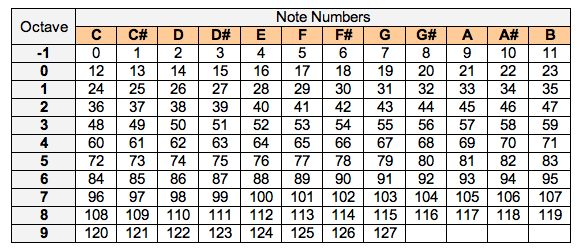
\includegraphics[width=0.7\linewidth]{nutymidi.jpg}
	\caption{Reprezentacja nut w formacie MIDI}
	\label{fig:fwxnbxgh4afzwe7}
\end{figure}

Nawiązując do powyżej tabeli, która reprezentuje dwa zdarzenia MIDI numery 67 oznaczają nutę G4. Kolejna zmienna o nazwie velocity przyjmuje wartości z zakresu (0-127). Jej zadaniem jest określenie siły danego dźwięku, inaczej mówiąc im mniejsza wartość zmiennej velocity tym dźwięk jest bardziej cichy. Pliki MIDI zawierają wszystkie istotne dane muzyczne, możliwe jest więc określenie prawdopodobieństwa przejścia z jednej nuty na drugą poprzez odpowiednią analizę pliku.

Innym dostępym formatem służącym do zapisu informacji o utworze muzycznym jest standard MusicXML$\pagenote{\texttt{http://www.musicxml.com/}}$. Jest to znacznikowy format prezentacji graficznej notacji muzycznej, który oparty jest na wzorcach dokumentowych DTD$\pagenote{\texttt{https://en.wikipedia.org/wiki/Document\_type\_definition}}$. Aby zrozumieć notację zapisu MusicXML wystarczy podstawowa znajomość języka XML, który jest dość powszechnie wykorzystywany. Format MusicXML jest wspierany przez ponad 230 programów służących do zapisu notacji muzycznej takich jak Finale\pagenote{\texttt{https://www.finalemusic.com/}}, Sibelius\pagenote{\texttt{http://www.avid.com/sibelius}} czy MusicScore\pagenote{\texttt{https://musescore.org/pl}}. Poniżej zostanie przedstawiona przykładowa struktura pliku MusicXML.

\begin{lstlisting}
<?xml version="1.0" encoding="UTF-8"?>
<!DOCTYPE score-partwise PUBLIC "-//Recordare//DTD MusicXML 3.1 Partwise//EN"
 "http://www.musicxml.org/dtds/partwise.dtd">
<score-partwise>
	<identification>
		<rights></rights>
		<encoding>
		<software></software>
		<encoding-date></encoding-date>
		</encoding>
	</identification>
	<part-list>
		<score-part id='P1'>
			<part-name>Track 1</part-name>
		</score-part>
	</part-list>
	<part id="P1">
		<measure number='1'>
			<atrributes>atrybut miary</atrributes>
			<note>
				<pitch>
					<step>C</step>
					<octave>4</octave>
				</pitch>
				<duration>96</duration>
				<type>whole</type>
			</note>
		</measure>
	</part>
</score-partwise>
\end{lstlisting}

Pierwsze trzy linijki definiują standard dokumentu XML. Plik partwise.dtd definiuje reprezentacje nut, plik timewise.dtd definiuje długości trwania nut. Następnie występuje główny tag o nazwie \xml{score-partwise}, którego dzieckiem jest tag \xml{identyfication}, którego zadaniem jest przechowywanie meta informacji o pliku. Tag \xml{score-part} reprezentuje ścieżkę utworu. Przykład powyżej posiada jedną ścieżkę, która jest opisana w tagu \xml{measure}. Poszczególna ścieżka posiada takie atrybuty jak tempo, rozmiar, tonację, metrum, klucz.


Bardzo ciekawym zastosowaniem łańcucha Markowa jest wykorzystanie go do generowania muzyki.
Weźmy dla przykładu dwie melodie (c,d,e,c,d,c,d,e,c,d) oraz (d,e,d,e,c,d,c,d,e,d). Podane melodie tworzą przestrzeń stanów $Q=\{c,d,e\}$. Macierz prawdopodobieństw jest obliczana według wzoru:

$$ a(q_{i},q_{j}) = \frac{\#(q_{i} \rightarrow q_{j})}{ \sum_{q_{k} \in Q} \#(q_{i} \rightarrow q_{k})} $$

gdzie $\#(q_{i} \rightarrow q_{j})$ jest ilością możliwych przejść ze stanu $q_{i}$ do stanu $q_{j}$. Macierz prawdopodobieństw wygląda następująco:
\[
a =
\begin{bmatrix}
a(c,c) & a(c,d) & a(c,e) \\
a(d,c) & a(d,d) & a(d,e) \\
a(e,c) & a(e,d) & a(e,e)
\end{bmatrix}
=
\begin{bmatrix}

0 & 1 & 0 \\
\frac{2}{7} & 0 & \frac{5}{7} \\
\frac{4}{5} & \frac{1}{5} & 0 

\end{bmatrix}
\] 

oraz:
$$ \pi = \Big( \pi(c), \pi(d), \pi(e) \Big) = \Big( \frac{1}{2}, \frac{1}{2}, 0 \Big) $$
Graf prawdopodobieństw dla powyższej macierzy przedstawia się w sposób następujący:
\begin{figure}[H]
\begin{center}
	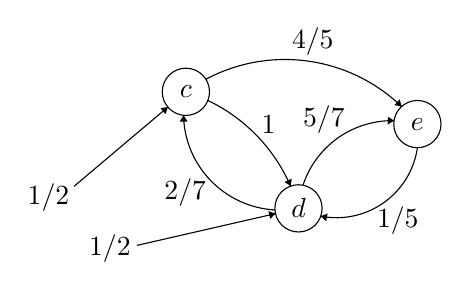
\begin{tikzpicture}[scale=0.1]
	\tikzstyle{every node}+=[inner sep=0pt]
	\draw [black] (29.7,-27.8) circle (3);
	\draw (29.7,-27.8) node {$c$};
	\draw [black] (59.1,-31.9) circle (3);
	\draw (59.1,-31.9) node {$e$};
	\draw [black] (44,-42.6) circle (3);
	\draw (44,-42.6) node {$d$};
	\draw [black] (32.239,-26.207) arc (118.06789:46.05406:21.343);
	\fill [black] (57.09,-29.67) -- (56.86,-28.76) -- (56.17,-29.48);
	\draw (45.82,-23.24) node [above] {$4/5$};
	\draw [black] (44.571,-39.663) arc (161.78715:88.85633:11.928);
	\fill [black] (56.14,-31.47) -- (55.35,-30.95) -- (55.33,-31.95);
	\draw (47.22,-33.16) node [above] {$5/7$};
	\draw [black] (59.105,-34.89) arc (-8.19129:-101.16523:10.381);
	\fill [black] (46.82,-43.6) -- (47.51,-44.24) -- (47.7,-43.26);
	\draw (56.61,-42.38) node [below] {$1/5$};
	\draw [black] (32.489,-28.898) arc (64.52751:23.50375:21.581);
	\fill [black] (43,-39.77) -- (43.14,-38.84) -- (42.22,-39.24);
	\draw (39.26,-31.91) node [right] {$1$};
	\draw [black] (41.014,-42.801) arc (-93.13852:-178.83021:12.293);
	\fill [black] (29.4,-30.78) -- (28.91,-31.59) -- (29.91,-31.57);
	\draw (32.32,-40.54) node [left] {$2/7$};
	\draw [black] (15.5,-39.8) -- (27.41,-29.74);
	\draw (14.95,-41.24) node [left] {$1/2$};
	\fill [black] (27.41,-29.74) -- (26.47,-29.87) -- (27.12,-30.63);
	\draw [black] (23.5,-47.3) -- (41.08,-43.27);
	\draw (22.75,-47.7) node [left] {$1/2$};
	\fill [black] (41.08,-43.27) -- (40.18,-42.96) -- (40.41,-43.94);
	\end{tikzpicture}
	\caption{Graf prawdopodobieństw równoważny z macierzą przejść}
\end{center}
\end{figure}
\subsection{Przykłady}

Alvin Lin w artykule pod tytułem: "Generating Musik Using Markov Chains"\pagenote{\texttt{https://medium.com/@omgimanerd/generating-music-using-markov-chains-40c3f3f46405}} opisał proces generowania muzyki z wykorzystaniem łańcucha Markowa na podstawie pliku MIDI. Wyniki jego rozważań można zobaczyć w praktyce uruchamiając przygotowane przez niego skrypty\pagenote{\texttt{https://github.com/omgimanerd/markov-music/}} napisane w języku Python. Rozważmy fragment utworu Dla Elizy kompozycji Ludwiga Van Beethovena, który zamieszczony jest poniżej. Na podstawie tego fragmentu będziemy chcieli wygenerować nowy fragment. Poniższy schemat nutowy zapisywany jest do pliku MIDI.

\begin{figure}[H]
	\centering
	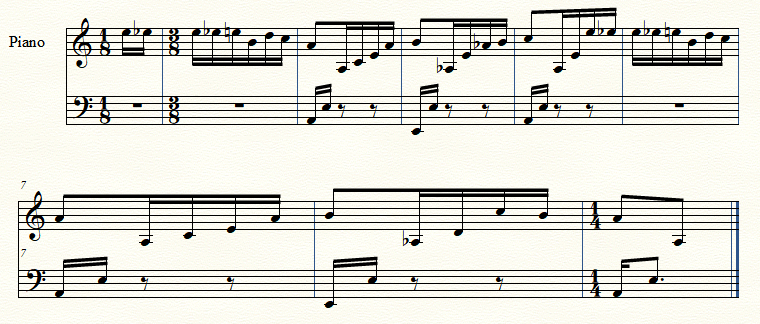
\includegraphics[width=0.7\linewidth]{przyklad_markov}
	\caption{Przykład melodii na podstawie której zostanie wygenerowana nowa.}
	\label{fig:przykladmarkov}
\end{figure}

Poniżej dokonano analizy pliku MIDI pod kontem poprawności. Jak widać poniżej plik MIDI zaczyna się z charakterystycznymi dla swojego formatu początkowymi nagłówkami.

\begin{figure}[H]
	\centering
	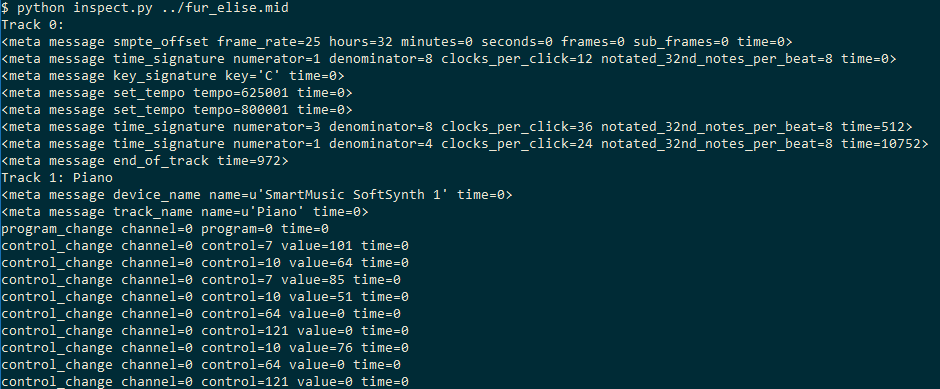
\includegraphics[width=0.5\linewidth]{analiza_midi}
	\caption{Fragment pliku MIDI po dokonaniu analizy}
	\label{fig:analizamidi}
\end{figure}

W dalszej części widać już poszczególne wartości nut razem z czasem oraz głośnością. 

\begin{figure}[H]
	\centering
	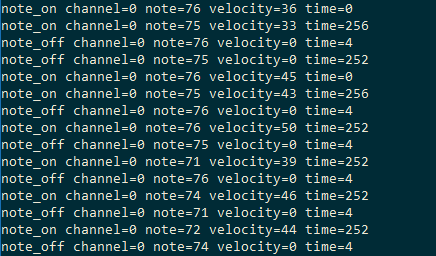
\includegraphics[width=0.5\linewidth]{nuty}
	\caption{Wartości nut}
	\label{fig:nuty}
\end{figure}


Do zbudowania łańcucha Markowa potrzebne będą informacje zawarte w liniach zaczynających się od $\mathnormal{note\_on}$ informacje tam zawarte mówią o numerze nuty i czasie. Należy więc z pliku MIDI wyodrębnić wszystkie dane zawierające wartość $\mathnormal{note\_on}$.


Dla każdej nuty, która gra z inną  w tym samym czasie zaokrąglany jest jej czas do najbliższych 250 milisekund. Zostało to przedstawione na grafie poniżej. 

\begin{figure}[H]
	\centering
	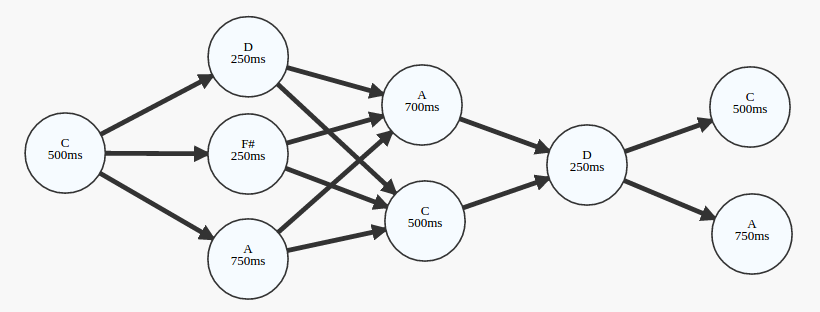
\includegraphics[width=0.5\linewidth]{graf_nuty}
	\caption{Nuty przedstawione w formie grafu skierowanego}
	\label{fig:grafnuty}
\end{figure}

Reprezentacją takiego grafu może być macierz sąsiedztwa. Między węzłami poszczególna nuta przechodzi w kolejną nutę. Dla uproszczenia uwzględniony został tylko czas trwania danej nuty i liczba przypadków w których została zmieniona na inną nutę. Macierz sąsiedztwa dla powyższego grafu przedstawia się w sposób następujący:

\begin{lstlisting}[caption={Macierz przejść},captionpos=b]
C (500 ms) | D (250 ms) | F# (250 ms) | A (750 ms)
C       0            2            1             1
D       2            0            0             2
F#      1            0            0             1
A       1            1            0             1
\end{lstlisting}

Ilustracja poniżej przedstawia macierz sąsiedztwa dla fragmentu utworu "Dla Elizy"

\begin{figure}[H]
	\centering
	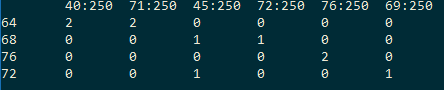
\includegraphics[width=0.7\linewidth]{macierz_dla_elizy}
	\caption{Macierz sąsiedztwa dla fragmentu utworu "Dla Elizy"}
	\label{fig:macierzdlaelizy}
\end{figure}

Numery komórek reprezentują nuty i czas trwania nuty do której nastąpiło przejście. Numery wierszy oznaczają nuty, z który odbyło się przejście. Każda pozycja w macierzy reprezentuje liczbę przypadków, gdy dana nuta została przeniesiona do innej. Do wygenerowania nowego utworu wybierana jest losowa nuta, następnie jest ona odnajdywana w macierzy. Kolejno z grupy wszystkich wyprowadzeń losowana jest następna nuta, jednak priorytet ma tutaj częstość przejść. Do wygenerowania nowych melodii posłużono się 50 iteracjami.

\begin{figure}[H]
	\centering
	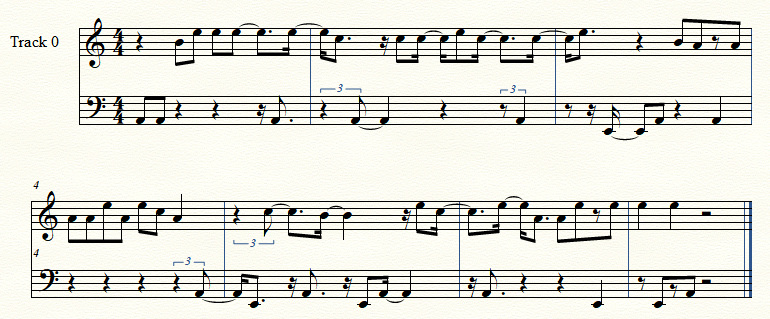
\includegraphics[width=0.7\linewidth]{przykad_1}
	\caption{Wyniki - przykład 1}
	\label{fig:przykad1}
\end{figure}

\begin{figure}[H]
	\centering
	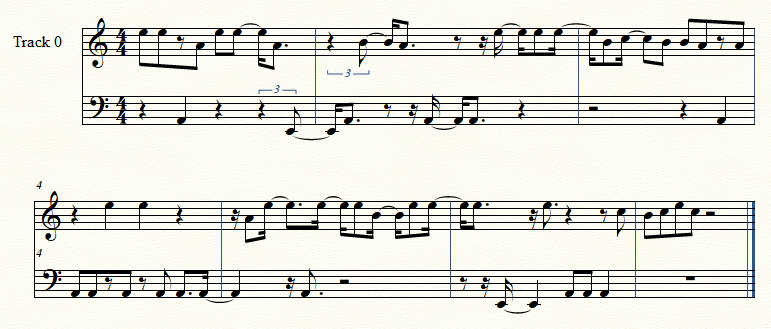
\includegraphics[width=0.7\linewidth]{przyklad_2}
	\caption{Wyniki - przykład 2}
	\label{fig:przyklad2}
\end{figure}

Niestety, ale melodie nie są przyjazne dla ucha. Chociaż, nie są też abstrakcyjne. Widocznie widać, że brakuje tutaj formy.  

Trochę inne, ale bardzo podobne podejście zaprezentował Justin Bozonier w artykule "Algorithm of the Week: Generate Music Algorithmically"\pagenote{\texttt{https://dzone.com/articles/algorithm-week-generate-music}}. W przykładzie wykorzystywana jest biblioteka PySynth\pagenote{\texttt{https://mdoege.github.io/PySynth/}} za pomocą, której autor generuje plik wav powstały z wcześniej wygenerowanych symboli nut w postaci A, B, C. W tym przykładzie nie jest wykorzystywany plik MIDI tylko zadaniem użytkownika jest ręczne wprowadzenie melodii na podstawie, której zostanie skonstruowana macierz przejść, a następnie nowa sekwencja nut. Poniżej został przedstawiony sposób definiowania sekwencji nut. Jak widać pierwszym elementem tablicy jest symbol nuty, a drugim czas trwania przy czym 1 oznacza całą nutę, 2 półnutę, 4 ćwierć nutę, 8 ósemkę i 16 szesnastkę. Cały kod dostępny jest w serwisie GitHub\pagenote{\texttt{http://github.com/jcbozonier/MarkovMusic/tree/master}}.

\begin{lstlisting}[caption={Sposób zapisu sekwencji nut},captionpos=b]
[...]
musicLearner.add(["c", 4])
musicLearner.add(["c", 4])
musicLearner.add(["d", 8])
musicLearner.add(["e", 4])
musicLearner.add(["f", 8])
musicLearner.add(["g", 2])
[...]
\end{lstlisting}

Jeszcze inne podejście zaprezentował użytkownik johmryan\pagenote{\texttt{https://github.com/johnmryan/music-generator}}, którego aplikacja składa się z dwóch części. Pierwsza część aplikacji to strona www, która zbiera od użytkownika ciąg nut w postaci symboli np. DBAGA oraz informacje o tym czy generowanie muzyki ma opierać się na łańcuchy Markowa pierwszego rzędu czy drugiego. Następnie dane wprowadzone przez użytkownika są wysyłane do skryptu napisanego w Pythonie. Skrypt na podstawie otrzymanej sekwencji tworzy nowe sekwencje i wysyła do witryny internetowej, która prezentuje wyniki. 
